\thispagestyle{empty}
%\thisfancypage{%đóng khung trang này
%\setlength{\fboxsep}{0pt}% 8pt là độ dày của đường viền
%\fbox}{} % phần nội dung sau là tương tự như đã làm
    \begin{tikzpicture}[remember picture,overlay,inner sep=0,outer sep=0]
      \draw[blue!70!black,line width=5pt] 
      ([xshift=-2cm,yshift=-2cm]current page.north east) coordinate (A)--
      ([xshift=2cm,yshift=-2cm]current page.north west) coordinate(B)--
      ([xshift=2cm,yshift=2cm]current page.south west) coordinate (C)--
      ([xshift=-2cm,yshift=2cm]current page.south east) coordinate(D)--cycle;

      \draw ([yshift=0.5cm,xshift=-0.5cm]A)-- ([yshift=0.5cm,xshift=0.5cm]B)--
      ([yshift=-0.5cm,xshift=0.5cm]B) --([yshift=-0.5cm,xshift=-0.5cm]B)--([yshift=0.5cm,xshift=-0.5cm]C)--([yshift=0.5cm,xshift=0.5cm]C)--([yshift=-0.5cm,xshift=0.5cm]C)-- ([yshift=-0.5cm,xshift=-0.5cm]D)--([yshift=0.5cm,xshift=-0.5cm]D)--([yshift=0.5cm,xshift=0.5cm]D)--([yshift=-0.5cm,xshift=0.5cm]A)--([yshift=-0.5cm,xshift=-0.5cm]A)--([yshift=0.5cm,xshift=-0.5cm]A);


      \draw ([yshift=-0.3cm,xshift=0.3cm]A)-- ([yshift=-0.3cm,xshift=-0.3cm]B)--
      ([yshift=0.3cm,xshift=-0.3cm]B) --([yshift=0.3cm,xshift=0.3cm]B)--([yshift=-0.3cm,xshift=0.3cm]C)--([yshift=-0.3cm,xshift=-0.3cm]C)--([yshift=0.3cm,xshift=-0.3cm]C)-- ([yshift=0.3cm,xshift=0.3cm]D)--([yshift=-0.3cm,xshift=0.3cm]D)--([yshift=-0.3cm,xshift=-0.3cm]D)--([yshift=0.3cm,xshift=-0.3cm]A)--([yshift=0.3cm,xshift=0.3cm]A)--([yshift=-0.3cm,xshift=0.3cm]A);

    \end{tikzpicture}
    
\begin{center}
    %\textbf{ }\\[10pt]
    \textbf{
    \begin{LARGE}
    ĐẠI HỌC BÁCH KHOA HÀ NỘI
    \end{LARGE} \\
    \begin{large}
    VIỆN TOÁN ỨNG DỤNG VÀ TIN HỌC
    \end{large} 
    }\\[12pt]
    \textbf{--------------------  *  ---------------------}\\[5pt]
    
\includegraphics[scale=0.8]{./image/logo.jpg}\\[12pt]
    {\fontsize{18pt}{1}\selectfont BÁO CÁO ĐỒ ÁN II}\\[1.5cm]
    {\fontsize{18pt}{1}\selectfont Đề tài: Phân tích, thiết kế hệ thống web quản lý học tập và đăng ký đồ án, thực tập của sinh viên}\\[12pt]

    \textbf{ }\\
    
  \end{center}
  \begin{tabular}{lllll}
      Giảng viên hướng dẫn&: & \textbf{TS. Ngô Quốc Hoàn} &&\\
      Sinh viên thực hiện&: & Nguyễn Văn Triển &&\\
      MSSV&: & 20195934 &&\\
      % Lớp: & Toán tin 02 - K64 & $\overline{\text{Chữ ký của GVHĐ}}$
      Lớp&: & Toán tin 02 - K64 && \textoverline{Chữ ký của GVHD}
      % \fontsize{16pt}{30}{$\overline{\text{Chữ ký của GVHD}}$}
  \end{tabular}\\
  % \hspace{4pt}\textbf{Chữ}
\vspace{2.5cm}
\begin{center}
{\fontsize{14pt}{1}\selectfont Hà Nội, tháng 03 năm 2023}
\end{center}
